\documentclass[runningheads]{llncs}
\usepackage[T1]{fontenc}
\usepackage{amsmath,amssymb,booktabs,graphicx,multirow}
\usepackage[hidelinks]{hyperref}
\setlength{\emergencystretch}{1.5em}
\begin{document}
\title{Hindsight Is Not Opportunity: Pre-Outcome Value in Risk-Constrained Label Acquisition with Delayed Feedback}
\titlerunning{Hindsight Is Not Opportunity}
\author{Anonymous Authors}
\authorrunning{Anonymous Authors}
\institute{Anonymous Institution}
\maketitle
\begin{abstract}
In credit and similar decision systems, labels are acquired through risky actions, outcomes arrive with delay, and a risk budget limits feasible label sets. Acquisition rules are often judged against the best set in hindsight, which overstates what any deployable rule can achieve. We propose an evaluation protocol that splits post-outcome headroom into an expected-value-of-perfect-information (foresight) term and a pre-outcome term, bracketed by plug-in and cross-fitted estimators when outcome probabilities are known. Using a mechanism-informed reference policy, DC-PRISM, we find: (i) in controlled worlds with directional pending information, 82--88\% of hindsight headroom is deployable across twelve generator variants, and DC-PRISM beats a quantity-maximizing risk reference in all of them; (ii) a common-family ablation attributes most of this gain to a target-weighted information proxy evaluated over a reference-anchored family, not to the conservative decision layer; (iii) foresight is a roughly constant $1.5$--$6.4\times10^{-3}$ Brier in every setting, so on real credit covariates, where deployable differences are of that order, 61--90\% of hindsight headroom is foresight, insensitive to family size; (iv) a power-driven replay on four credit cohorts shows gains over quantity references on two cohorts, losses to information-greedy baselines on two others, and realized risk far below the budget.
\keywords{Selective labels \and Risk-constrained acquisition \and Delayed feedback \and Value of information \and Credit risk}
\end{abstract}

\section{Introduction}
\label{sec:intro}
A lender observes repayment only for applications it approves, so the data available for future learning depend on earlier decisions~\cite{lakkaraju2017selective,wei2021selective}. Each approval is also an exposure to loss, and outcomes arrive with delay. Data-centric decision pipelines face this structure whenever labels are bought with actions rather than annotation effort: a risk budget, incomplete coverage, and information that is committed but still pending.

Active learning and experimental design select observations by their expected contribution to prediction~\cite{cohn1996active,chaloner1995bayesian,settles2009active}; recent criteria target Fisher information, predictive information or downstream loss~\cite{ash2021fishing,bickfordsmith2023prediction,huang2026loss}. Under a risk budget one informative but exposed observation can displace several cheap ones, so composition and quantity trade off directly, and pending outcomes change the comparison again because information along some directions is already on its way.

How should acquisition rules be \emph{evaluated} in this setting? A common diagnostic compares the chosen set with the set that turned out best once outcomes were revealed. That comparison mixes two things: value that a rule could have realized from the information at hand, and value that requires knowing the hidden training labels. In decision analysis the second is the expected value of perfect information (EVPI)~\cite{howard1966information,raiffa1961applied}, and selecting the best of several noisy estimates is biased upward by the optimizer's curse~\cite{smith2006optimizer}. Neither observation is new. What is missing is an evaluation protocol that makes the distinction measurable for risk-constrained acquisition and shows how large each part is in practice.

\paragraph{Contributions.}
\begin{itemize}
\item \textbf{Evaluation protocol.} We decompose post-outcome headroom over a visible candidate family into an EVPI-type foresight term and a pre-outcome term, give a plug-in/cross-fitted bracket for the latter, and show that the resulting shares are stable in the size of the family (Sec.~\ref{sec:opportunity}, \ref{sec:controlled}).
\item \textbf{Mechanism.} A same-state quantity--composition decomposition and a two-direction example in which pending information reverses the preferred set under an unchanged budget; they motivate the design, although our experiments do not isolate the pending mechanism (Sec.~\ref{sec:mechanism}, \ref{sec:controlled}).
\item \textbf{Layered evidence.} Pre-registered studies on controlled worlds (including twelve generator variants and a common-family ablation of the decision rule), on real credit covariates with paired coverage interventions, and in power-driven delayed replay on four credit cohorts with eight comparators (Secs.~\ref{sec:controlled}--\ref{sec:replay}).
\end{itemize}
DC-PRISM, the policy used as an instrument, follows from the mechanism (Sec.~\ref{sec:policy}). We do not claim that it outperforms simple information-based baselines on real data; the experiments show where it does and does not, and which of its parts matter.

\section{Setting}
\label{sec:setting}
At round $t$, a learner observes labeled history $D_t$, the covariates of pending acquisitions $O_t$, an unlabeled candidate pool $C_t$ and target covariates $Q_t$. Candidate $i$ has a visible exposure $e_i\geq0$ and a binary adverse outcome $Y_i$ revealed only after acquisition and a feedback delay. A legal policy chooses $S_t\subseteq C_t$ using the visible information $\mathcal H_t$; outcomes in $O_t$ and $C_t$ stay hidden. Learning is measured with the Brier score~\cite{brier1950verification}. For a fixed state, $L(S;Y)$ denotes test loss after fitting on $D\cup O\cup S$, where $Y$ collects the hidden training outcomes of $O$ and $S$.

\paragraph{Risk-feasible sets.} Let $q_i\in[0,1]$ be a risk score available at selection, $\ell=\log(1/\alpha)$, and $\phi(q)=q(1-q)$ for $q\le1/2$, $\phi(q)=1/4$ otherwise. For nonempty $S$,
\begin{equation}
 R_\alpha(S)=\sum_{i\in S}e_iq_i+\Big(2\ell\sum_{i\in S}e_i^2\phi(q_i)\Big)^{1/2}+\frac{\ell}{3}\max_{i\in S}e_i,
 \label{eq:envelope}
\end{equation}
$R_\alpha(\varnothing)=0$, and $\mathcal A_t=\{S\subseteq C_t:R_\alpha(S)\le B_t\}$. If, conditional on $\mathcal H_t$, the selected outcomes are independent Bernoulli variables with $p_i\le q_i$, a sub-gamma bound~\cite{boucheron2013concentration} gives $\Pr\{\sum_{i\in S}e_iY_i>R_\alpha(S)\mid\mathcal H_t\}\le\alpha$. Our scores do not guarantee $p_i\le q_i$, so we use~\eqref{eq:envelope} as the operational feasible region shared by all policies and report realized exceedance empirically (Secs.~\ref{sec:controlled}, \ref{sec:replay}).

\paragraph{Risk scores.} With the $\ell_2$-regularized logistic fit $\widehat\theta$ on $D_t$, let $u$ be the one-sided 95\% Wilson upper bound~\cite{wilson1927probable} on the default rate of the upper half of $D_t$ by fitted risk, and $\bar p$ the mean fitted risk of that half. The logit shift $\delta=\mathrm{clip}(\mathrm{logit}\,u-\mathrm{logit}\,\bar p,0.15,1.15)$ is added to 40 Laplace draws $\bar x_i^\top\theta^{(m)}$, $\theta^{(m)}\sim\mathcal N(\widehat\theta,H_D^{-1})$, and $q_i$ is the logistic transform of their $0.9875$ quantile.

\paragraph{Quantity reference.} The reference $M_K\in\mathcal A_t$ maximizes cardinality and breaks ties by smaller envelope; $K=|M_K|$. Pools of at most 16 candidates are enumerated. Larger pools use a search stratified by the exposure ceiling $\max_{i\in S}e_i$: for each distinct ceiling, sorting means and variances separately gives an upper bound on the feasible cardinality, and five mixed orderings give feasible prefixes, followed by one-for-one swaps that lower the envelope. This takes $O(n^2\log n+nK^2)$ time for $n$ candidates and certifies the cardinality whenever the bound is attained. This happened in 1{,}320 of the 1{,}408 fresh offline states below, including 63 of 64 pools of 48 candidates with $K=12$; in the remaining 88 (85 of them in controlled worlds with negative risk--information coupling) the bound exceeds the found cardinality by one label.

\section{Mechanism and Evaluation Protocol}
\label{sec:mechanism}
\subsection{Quantity and Composition}
For a selected $S$ with $|S|=k\le K$, let $M_k$ be a feasible risk-ranked reference of size $k$ (with $M_K$ reused when $k=K$). From the same $D\cup O$ and realized outcomes,
\begin{equation}
\begin{gathered}
 Q_k=L(M_k;Y)-L(M_K;Y),\qquad C_k=L(M_k;Y)-L(S;Y),\\
 J=L(M_K;Y)-L(S;Y)=C_k-Q_k.
\end{gathered}
 \label{eq:decomposition}
\end{equation}
The identity is elementary; its use is diagnostic. $Q_k$ compares two risk references of different size and $C_k$ compares equally sized sets, so $J>0$ with $Q_k\approx0$ attributes a gain to composition rather than to taking fewer labels.

\subsection{Directional Pending Information}
Consider a two-parameter linear Gaussian model with precision $P=\operatorname{diag}(h_1,h_2)$, target weights $\operatorname{diag}(g_1,g_2)$ and loss $\sum_jg_j/P_{jj}$. Pending observations add precision $o\ge0$ along direction~1; the quantity reference adds $a$ along direction~1, a smaller alternative adds $b$ along direction~2, and both stay feasible. The alternative's gain is
$J(o)=\frac{g_2b}{h_2(h_2+b)}-\frac{g_1a}{(h_1+o)(h_1+o+a)}$, strictly increasing in $o$, and with $v_2=g_2b/[h_2(h_2+b)]$ the alternative is preferred exactly when
\begin{equation}
 o>o^*=\tfrac12\big(-a+\sqrt{a^2+4g_1a/v_2}\big)-h_1 .\label{eq:threshold}
\end{equation}
With $h_j=g_j=1$, $a=4$, $b=1$, $\alpha=0.1$ and $q=0.1$, exposures $0.1$ per reference label and $0.1624$ for the alternative give both actions envelope $B\approx0.2455$ and no feasible mixture; the reference is preferred at $o=0$ (loss $1.20$ versus $1.50$), the alternative at $o=1$ ($1.17$ versus $1.00$), and $o^*\approx0.464$. The calculation is simple but fixes a design requirement: value candidates against history plus pending covariates.

\subsection{Hindsight Versus Pre-Outcome Opportunity}
\label{sec:opportunity}
Fix $\mathcal H$ and a finite family $\mathcal F$ of sets constructed from visible information and containing $M=M_K$. Let $\bar L(S;Y)$ be $L(S;Y)$ with test-label noise integrated out, keeping the hidden training labels $Y$. Define
\begin{align}
 H_{\mathrm{post}}&=\mathbb E\big[\bar L(M;Y)-\min_{S\in\mathcal F}\bar L(S;Y)\mid\mathcal H\big],\\
 H_{\mathrm{pre}}&=\mathbb E[\bar L(M;Y)\mid\mathcal H]-\min_{S\in\mathcal F}\mathbb E[\bar L(S;Y)\mid\mathcal H].
\end{align}
For any legal policy $\pi$ choosing within $\mathcal F$ with expected gain $\Gamma_\pi=\mathbb E[\bar L(M;Y)-\bar L(\pi;Y)\mid\mathcal H]$,
\begin{equation}
 H_{\mathrm{post}}-\Gamma_\pi=\underbrace{H_{\mathrm{post}}-H_{\mathrm{pre}}}_{\text{foresight}}+\underbrace{H_{\mathrm{pre}}-\Gamma_\pi}_{\text{pre-outcome selection gap}} .\label{eq:opportunity}
\end{equation}
The foresight term is the EVPI of the hidden training labels for the decision ``which $S\in\mathcal F$''~\cite{howard1966information,raiffa1961applied}; it is nonnegative because $\mathbb E\min\le\min\mathbb E$, and no deployable policy can close it. Our contribution is not this inequality but its use as an evaluation protocol: a rule should be judged against $H_{\mathrm{pre}}$, and hindsight comparisons with the realized best set, which estimate $H_{\mathrm{post}}$, overstate deployable opportunity by exactly the EVPI.

\paragraph{Estimation.} When the outcome probabilities $p$ are known, we draw $R=128$ replicates $Y^{(r)}$ of the hidden training labels and evaluate every $S\in\mathcal F$ on all replicates with common draws. $H_{\mathrm{post}}$ is then estimated without bias. The plug-in $\widehat H_{\mathrm{pre}}$, which minimizes the replicate mean, is biased upward because it selects on noise, an instance of the optimizer's curse~\cite{smith2006optimizer,cawley2010overfitting}. A two-fold cross-fitted estimate~\cite{chernozhukov2018double}, which chooses $S^\star$ on even replicates and evaluates it on odd ones (and vice versa), is biased downward. Together they bracket $H_{\mathrm{pre}}$, and $H_{\mathrm{post}}-\widehat H_{\mathrm{pre}}^{\text{plug-in}}$ is a conservative estimate of foresight. Because both terms are defined relative to $\mathcal F$, we report how they change with $|\mathcal F|$ (Sec.~\ref{sec:controlled}).

\section{DC-PRISM: A Mechanism-Informed Reference Policy}
\label{sec:policy}
DC-PRISM values a feasible set by the target-weighted Brier reduction it would add to history and pending information, and compares it with the quantity reference. With $\bar x=(1,x^\top)^\top$, $p_\theta(x)=\sigma(\bar x^\top\theta)$ and $w_\theta=p_\theta(1-p_\theta)$, let
\begin{gather*}
 H_{D+O}(\theta)=\Lambda+\!\!\sum_{i\in D\cup O}\!\!w_\theta(x_i)\bar x_i\bar x_i^\top,\qquad
 A_S(\theta)=\sum_{i\in S}w_\theta(x_i)\bar x_i\bar x_i^\top,\\
 W_Q(\theta)=\tfrac1{|Q|}\sum_{j\in Q}w_\theta(x_j)^2\bar x_j\bar x_j^\top,
\end{gather*}
and
\begin{equation}
 V_\theta(S)=\operatorname{tr}\!\big[W_Q(\theta)\{H_{D+O}(\theta)^{-1}-(H_{D+O}(\theta)+A_S(\theta))^{-1}\}\big].\label{eq:value}
\end{equation}
$V_\theta$ is a local quadratic proxy for target Brier reduction in the spirit of transductive design and predictive-information acquisition~\cite{yu2006transductive,bickfordsmith2023prediction}; pending covariates enter $H_{D+O}$ without their labels, which is the discounting in~\eqref{eq:threshold}.

\paragraph{Decision rule.} The candidate family $\mathcal F_t$ contains $M_K$, value-per-envelope-cost prefixes, value-ranked prefixes and exchanges that keep part of $M_K$, all checked against~\eqref{eq:envelope}. For $m=1,\dots,20$ draws $\theta^{(m)}\sim\mathcal N(\widehat\theta,H_D^{-1})$~\cite{mackay1992practical}, candidate curvature is damped by $\exp[-0.45\{\bar x_i^\top(\theta^{(m)}-\widehat\theta)\}^2]$ and, with $a_m=\max\{V_m(M_K),10^{-6}\}$,
\begin{equation}
 Z(S)=\operatorname{quantile}_{0.2}\Big\{\tanh\frac{V_m(S)-a_m}{2.5a_m}\Big\}_m-0.22\,\frac{(K-|S|)_+}{\max(K,1)} .\label{eq:score}
\end{equation}
DC-PRISM chooses $\arg\max Z$ if $Z>0.08$ and $M_K$ otherwise. We call the draw quantile, damping, reference normalization, penalty and gate the \emph{conservative layer}. Its constants were inherited from an earlier version of the package and fixed before any study reported here; we cannot certify that they were chosen without the controlled generator in view, which is why Sec.~\ref{sec:controlled} perturbs the generator and the constants. Building the family costs $O(Kn\,d^2)$ and scoring it $O(20\,|\mathcal F_t|\,(d^3+Kd^2))$ for $d$ features; a selection takes 53\,ms on average (maximum 0.18\,s) with $n=24$ and 0.09--0.11\,s with $n=48$ on one CPU core, against 5\,ms for the greedy baselines.

\paragraph{Comparators.} All policies share the state, $q$, the numerical budget and~\eqref{eq:envelope}. \emph{Safe-MinRisk} returns $M_K$. \emph{Fixed count} selects a fixed fraction of $K$ labels by point value. \emph{Fisher-cost} greedily packs by single-observation parameter-variance reduction per exposure cost. Four baselines pack greedily until no feasible candidate remains: \emph{Random}; \emph{Uncertainty}, ordered by $\widehat p(1-\widehat p)$~\cite{lewis1994sequential}; \emph{BAIT-greedy}, forward greedy on $\operatorname{tr}(F_Q(H_{D+O}+A_S)^{-1})$ with the pool Fisher matrix $F_Q$~\cite{ash2021fishing}; and \emph{TargetVar-greedy}, forward greedy on~\eqref{eq:value}, an EPIG-style Laplace approximation~\cite{bickfordsmith2023prediction} that uses DC-PRISM's proxy without its family or conservative layer. Greedy packing is the standard approach for such objectives under knapsack-type constraints~\cite{krause2005near,sviridenko2004note}.

\section{Controlled Evidence}
\label{sec:controlled}
\paragraph{Design.} Each world has six features, 80 historical labels with narrow coverage, 22 pending acquisitions, 24 candidates, 180 target and 240 test points. Candidates fall into low-risk core observations, pending-aligned observations, observations on two further predictive directions, and auxiliary-tail observations whose outcomes follow a regime switch that a logistic model cannot represent. The default world places all pending acquisitions on one direction and couples information positively with exposure. All selections are locked before any hidden label is read. Every study fixed its world counts, seeds, comparison families and a material-effect threshold of $5\times10^{-4}$ Brier before running; protocols and code were frozen in a version-controlled repository before execution (the final batch at an anonymized commit hash, listed in the supplement). We report paired means with 95\% Bonferroni simultaneous $t$ intervals and Holm-adjusted tests~\cite{holm1979simple} within each family; all differences below are in units of $10^{-3}$ Brier.

\paragraph{Realized gains and their composition.} In 128 archived worlds DC-PRISM attains Brier $0.1202$ with $3.27$ labels, against $0.1367$ for Safe-MinRisk with six labels and $0.1367$ for a fixed-count rule that takes $\mathrm{round}(0.75K)=4$ labels (paired excess $16.49$, 95\% CI $[10.97,22.00]$). The decomposition~\eqref{eq:decomposition} gives $C_k=16.26$, $Q_k=-0.19$ and $J=16.45$: the gain is compositional, and the smaller risk reference is no worse than the larger one.

\paragraph{Fresh worlds, ex-ante endpoint.} In 128 fresh worlds we score every policy by expected Brier, integrating test-label noise exactly and training-label noise over 128 replicates (Table~\ref{tab:controlled}; fixed count here takes $\lceil0.75K\rceil=5$ labels). DC-PRISM has the lowest loss, and its gains over Safe-MinRisk ($12.2$, $[7.6,16.8]$), Fisher-cost, Random and fixed count are material. Against Uncertainty, BAIT-greedy and TargetVar-greedy the gains are $2.7$--$4.2$ with intervals that include zero. A second fresh set (Study F) gives $15.9$ $[8.5,23.3]$ and $5.4$ $[1.0,9.9]$ over Safe-MinRisk and TargetVar-greedy.

\begin{table}[t]
\caption{Fresh controlled worlds (128): ex-ante expected Brier, mean labels, and DC-PRISM's gain with 95\% simultaneous intervals ($\times10^{-3}$; positive favors DC-PRISM).}
\label{tab:controlled}
\centering\small
\begin{tabular}{lrrr}
\toprule
Policy & Expected Brier & Labels & Gain of DC-PRISM \\
\midrule
Safe-MinRisk & 0.1384 & 6.00 & $12.2$ [$7.6$, $16.8$] \\
Fixed count & 0.1358 & 5.00 & $9.6$ [$5.1$, $14.2$] \\
Random & 0.1359 & 3.54 & $9.7$ [$5.1$, $14.4$] \\
Uncertainty & 0.1304 & 2.81 & $4.2$ [$-0.8$, $9.2$] \\
Fisher-cost & 0.1440 & 2.67 & $17.8$ [$13.2$, $22.4$] \\
BAIT-greedy & 0.1289 & 2.22 & $2.7$ [$-1.3$, $6.7$] \\
TargetVar-greedy & 0.1290 & 2.19 & $2.8$ [$-1.2$, $6.9$] \\
DC-PRISM & \textbf{0.1262} & 3.12 & -- \\
\bottomrule
\end{tabular}
\end{table}

\paragraph{Generator perturbation.} Because the default world was designed around the mechanism, we vary it (Study G, 64 fresh worlds per cell): pending overlap \{high, medium, low\} $\times$ risk--information coupling \{positive, neutral, negative\}, the tail regime replaced by the logistic link, and a doubled pool of 48 candidates with $K=6$ and $K=12$. DC-PRISM's gain over Safe-MinRisk is material in all twelve cells ($10.8$--$31.4$, Table~\ref{tab:perturb}), including the world without a misspecified tail and the larger pools. Its gain over TargetVar-greedy is material in five of the six cells with neutral or negative risk--information coupling ($9.7$--$17.9$) and indeterminate in the other seven, including all cells with positive coupling. The pre-outcome share of hindsight headroom stays between 82\% and 88\% in every cell. The pending mechanism of Sec.~\ref{sec:mechanism}, however, is not what the controlled gain isolates: the gain \emph{grows} as pending overlap falls ($11.5$--$16.9$ with high overlap, $28.8$--$31.4$ with low overlap), and in an earlier common-family study removing pending covariates from the proxy changed loss by only $0.9$ $[-1.0,2.8]$. Pending-awareness is thus a design rationale that our evidence neither confirms nor refutes.

\begin{table}[t]
\caption{Generator perturbation (64 worlds per cell; $\times10^{-3}$ expected Brier). Gains of DC-PRISM with 95\% simultaneous intervals over the 24-test family, bold where material; ``pre'' is $\widehat H_{\mathrm{pre}}^{\text{plug-in}}/H_{\mathrm{post}}$.}
\label{tab:perturb}
\centering\scriptsize
\setlength{\tabcolsep}{3pt}
\begin{tabular}{lrrrr}
\toprule
Cell (overlap / coupling) & vs Safe-MinRisk & vs TargetVar-greedy & $H_{\mathrm{post}}$ & pre \\
\midrule
High / positive (default) & {\bfseries\boldmath $11.5$ [$4.7$, $18.4$]} & $4.6$ [$-0.1$, $9.3$] & 21.6 & 85\% \\
High / neutral & {\bfseries\boldmath $16.9$ [$7.6$, $26.2$]} & {\bfseries\boldmath $9.7$ [$3.1$, $16.2$]} & 26.6 & 87\% \\
High / negative & {\bfseries\boldmath $14.3$ [$6.9$, $21.7$]} & {\bfseries\boldmath $10.3$ [$3.3$, $17.3$]} & 21.7 & 86\% \\
Medium / positive & {\bfseries\boldmath $12.6$ [$4.0$, $21.2$]} & $4.5$ [$-1.2$, $10.2$] & 22.4 & 82\% \\
Medium / neutral & {\bfseries\boldmath $13.6$ [$5.5$, $21.6$]} & {\bfseries\boldmath $13.1$ [$4.9$, $21.2$]} & 23.4 & 83\% \\
Medium / negative & {\bfseries\boldmath $12.9$ [$1.1$, $24.7$]} & {\bfseries\boldmath $9.9$ [$2.8$, $17.0$]} & 22.3 & 83\% \\
Low / positive & {\bfseries\boldmath $28.8$ [$16.3$, $41.3$]} & $3.8$ [$-3.6$, $11.2$] & 47.4 & 86\% \\
Low / neutral & {\bfseries\boldmath $30.7$ [$17.6$, $43.8$]} & $7.2$ [$-2.3$, $16.8$] & 47.0 & 87\% \\
Low / negative & {\bfseries\boldmath $31.4$ [$17.1$, $45.6$]} & {\bfseries\boldmath $17.9$ [$7.8$, $28.0$]} & 46.3 & 88\% \\
Default, no tail regime & {\bfseries\boldmath $10.8$ [$5.4$, $16.2$]} & $3.0$ [$-2.3$, $8.4$] & 19.9 & 84\% \\
Default, 48 candidates, $K=6$ & {\bfseries\boldmath $14.9$ [$5.2$, $24.6$]} & $3.4$ [$-3.7$, $10.4$] & 24.0 & 87\% \\
Default, 48 candidates, $K=12$ & {\bfseries\boldmath $12.5$ [$4.0$, $21.1$]} & $4.5$ [$-0.4$, $9.3$] & 21.0 & 88\% \\
\bottomrule
\end{tabular}
\end{table}

\paragraph{What drives the gain? A common-family ablation.} The comparison with TargetVar-greedy confounds the conservative layer with the candidate family. In Study F (128 fresh worlds) we therefore apply each rule to the same family $\mathcal F^+$, DC-PRISM's family plus the TargetVar-greedy set. The point proxy's own maximizer, $\arg\max_{\mathcal F^+}V_{\widehat\theta}$, already gains $13.1$ $[6.1,20.2]$ over Safe-MinRisk; the full conservative layer on the same family gains $16.1$, an increment of $3.0$ $[-0.2,6.2]$ that is not confirmed. Within the layer, evaluating~\eqref{eq:score} over parameter draws rather than at $\widehat\theta$ alone matters ($6.3$ $[1.0,11.6]$), whereas the low quantile ($2.3$ $[-0.9,5.5]$) and the penalty and gate ($-0.2$ $[-1.3,0.9]$) do not. Using the layer only as a veto on the greedy set adds nothing ($-0.2$ $[-2.1,1.8]$). Most of the controlled gain is therefore delivered by the target-weighted proxy evaluated over a reference-anchored family of sets, which on average also beats forward greedy selection on the same proxy ($13.1$ against $10.5$); the conservative layer's net contribution is positive in expectation but unconfirmed.

\paragraph{Opportunity and family size.} In the fresh worlds $H_{\mathrm{post}}=22.2$ and $H_{\mathrm{pre}}\in[18.4,18.5]$: 83\% of hindsight headroom is deployable, and DC-PRISM captures two thirds of it. Since both quantities are defined relative to $\mathcal F$, Study E enlarges each family with 64 random feasible sets and recomputes them on random sub-families of fixed size containing $M_K$, using the same label replicates (Fig.~\ref{fig:family}). Enlarging the family from about 27 to 88 sets raises $H_{\mathrm{post}}$ from $22.2$ to $27.6$ but raises $H_{\mathrm{pre}}$ in proportion, so the pre-outcome share stays at 83.5\%; on random sub-families it is between 80\% and 83\% for every size from 2 to 80. Replacing the structured family by random feasible sets of the same size gives 82.8\%. The share is thus a property of the state rather than of the family's size or construction.

\begin{figure}[t]
 \centering
 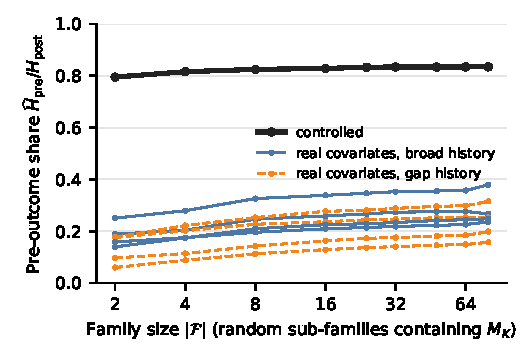
\includegraphics[width=0.62\linewidth]{figures/supplement_v5_family_size.pdf}
 \caption{Pre-outcome share of hindsight headroom on random sub-families of fixed size that contain $M_K$ (Study E; 128 controlled worlds and 64 pairs per real-covariate arm, the same label replicates throughout). Each thin line is one real-covariate arm.}
 \label{fig:family}
\end{figure}

\paragraph{Constants and risk.} Changing any single constant (quantile $0.1$--$0.5$, penalty $0$--$0.44$, gate $0$--$0.16$, damping $0$--$0.9$, tanh scale $1.25$--$5$) changes expected loss by at most $1.3$, and the gate never by more than $0.03$. Since $p$ is known in these worlds, we computed the exact probability that a selected set's realized adverse exposure exceeds its envelope: it is at most $2.8\times10^{-3}$ for every policy and state, far below $\alpha=0.1$, although $q_i\ge p_i$ holds for all members of only 95--99\% of selected sets, depending on the policy.

\section{Real Covariates: Where the Opportunity Goes}
\label{sec:realx}
\paragraph{Design.} We keep the real covariates of HMEQ and LendingClub and generate outcomes from a known logistic or nonlinear logit ($p(x)=\sigma(-0.8+x^\top\beta)$, optionally plus $0.5\sin x_2+0.35x_3x_4$), so that $H_{\mathrm{pre}}$ is measurable. In each of 64 fresh pairs per setting, a 240-record reservoir supplies two histories: \emph{broad} (80 random records) and \emph{gap} (the 80 lowest on the second feature). Candidates, pending and target records, labels, preprocessing, risk scores, budget, reference and family are identical across arms, so the pair isolates history coverage.

\paragraph{Most hindsight headroom is foresight.} $H_{\mathrm{post}}$ is an order of magnitude smaller than in controlled worlds and mostly foresight (Table~\ref{tab:realx}): the pre-outcome share is 10--39\% across the eight arms (cross-fitted to plug-in), against 82--88\% in every controlled variant. Families are of similar size in both settings (22--23 against 27 sets on average), and the gap persists at every matched size (Fig.~\ref{fig:family}): at $|\mathcal F|=16$ the real-covariate shares are 13--34\%. Enlarging the families to 81--84 sets changes them by at most 6 points, and on random sub-families they rise slightly rather than fall with $|\mathcal F|$, the opposite of what an artifact of family size would produce. In absolute terms foresight is similar everywhere: $1.5$--$6.4$ in all 21 controlled and real-covariate groups, against a deployable part that ranges from $0.3$ to $41$. Hindsight comparisons therefore mislead most when the true differences between feasible sets are of the order of this label-noise EVPI, as on every real-covariate arm. Coverage gaps more than double $H_{\mathrm{post}}$ (from $1.9$--$2.4$ to $4.9$--$6.4$) and raise $H_{\mathrm{pre}}$ to at most $1.9$; foresight is materially positive in all nine groups.

\begin{table}[t]
\caption{Real-covariate states (64 pairs per setting; $\times10^{-3}$ expected Brier). $H_{\mathrm{pre}}$ is bracketed by the cross-fitted and plug-in estimates. ``Proxy'' is the gain of $\arg\max_{\mathcal F}V_{\widehat\theta}$ over the evaluation family; $\rho$ is the Spearman correlation between $V_{\widehat\theta}$ and the true ex-ante gain across $\mathcal F$; ``$=M_K$'' is the share of states where DC-PRISM returns the reference.}
\label{tab:realx}
\centering\small
\setlength{\tabcolsep}{2.5pt}
\begin{tabular}{llrrrrrr}
\toprule
Setting & Arm & $H_{\mathrm{post}}$ & $H_{\mathrm{pre}}$ & DC gain & Proxy gain & $=M_K$ & $\rho$ \\
\midrule
HMEQ, logistic & broad & 2.19 & [0.48, 0.58] & 0.04 & 0.11 & 86\% & 0.27 \\
 & gap & 6.37 & [1.49, 1.87] & $-0.04$ & 1.13 & 88\% & 0.64 \\
HMEQ, nonlinear & broad & 2.43 & [0.85, 0.94] & $-0.02$ & 0.10 & 84\% & 0.31 \\
 & gap & 5.83 & [1.51, 1.89] & 0.10 & 0.54 & 95\% & 0.55 \\
LC, logistic & broad & 2.00 & [0.29, 0.39] & 0.04 & 0.03 & 92\% & 0.33 \\
 & gap & 4.88 & [0.51, 0.83] & 0.02 & 0.13 & 92\% & 0.69 \\
LC, nonlinear & broad & 1.89 & [0.31, 0.41] & 0.01 & $-0.01$ & 88\% & 0.14 \\
 & gap & 5.16 & [0.64, 0.96] & 0.04 & 0.05 & 95\% & 0.65 \\
\midrule
Controlled & -- & 22.21 & [18.38, 18.53] & 12.19 & 10.69 & 4\% & $-0.01$ \\
\bottomrule
\end{tabular}
\end{table}

\paragraph{Locating the pre-outcome gap.} DC-PRISM's ex-ante gain is within $\pm0.1$ in every arm, so its selection gap is almost all of $H_{\mathrm{pre}}$. Ranking the evaluation family by $V_\theta$ at the fitted $\widehat\theta$ and at the population parameter $\theta_{\mathrm{pop}}$ (the KL projection of the true $p$ onto the logistic class), neither the parameter effect (means $0.02$--$0.61$) nor the remaining approximation gap ($0.09$--$0.40$) is material in any of the 16 registered real-covariate tests. Under coverage gaps the proxy ranks the family well ($\rho=0.55$--$0.69$), and its maximizer captures 76\% of the cross-fitted $H_{\mathrm{pre}}$ in HMEQ-logistic but only 8--36\% in the other gap settings. In the controlled worlds the proxy ranks the whole family poorly ($\rho\approx0$) yet its maximizer gains $10.7$: it identifies the few best sets without ordering the rest. Ranking at $\theta_{\mathrm{pop}}$ is materially worse there ($-11.2$ $[-15.7,-6.6]$), and the approximation gap $H_{\mathrm{pre}}^{\text{cf}}-\Gamma(\theta_{\mathrm{pop}})=18.4-(-0.5)=18.9$ $[14.2,23.5]$ is material, consistent with the misspecified tail regime.

\paragraph{The conservative layer on real covariates.} The fresh ablation of Study F repeats this picture. DC-PRISM returns $M_K$ in 86--98\% of real-covariate states. In HMEQ-logistic with a coverage gap, the proxy maximizer on $\mathcal F^+$ gains $1.40$ $[0.34,2.46]$ over the reference and the conservative layer forgoes $1.34$ $[0.38,2.30]$ of it; in the other seven arms both are within $\pm0.65$ and no contrast is decisive. Combined with the controlled ablation, the evidence that conservatism \emph{helps} is weak (an unconfirmed $+3.0$ in controlled worlds), whereas the evidence that it can \emph{cost} deployable value where the proxy is reliable is clearer but limited to one of eight arms. Throughout, the amounts at stake on real covariates are small: at most about $2\times10^{-3}$ Brier is deployable in our settings.

\section{Delayed Replay on Real Labels}
\label{sec:replay}
\paragraph{Protocol.} We replay ten rounds on processed HMEQ, LendingClub, PPDai and UCI Credit cohorts with six features and recorded binary outcomes~\cite{sasHMEQ,lendingclubSource,ppdaiSource,he2018ensemble,yeh2009comparison}. Each seed reserves 1{,}000 test rows, 600 target rows and a 600-row history window from which 68 initial records are taken. Each round offers 24 candidates and 14 ordinary acquisitions. Exploration labels arrive one round after selection and ordinary labels two rounds after; Brier loss, ROC-AUC and log-loss are measured at the start of each round, after due releases, and averaged over the ten rounds (ALC). Preprocessing is fitted on the initial history, and the numerical budget is fixed across policies from the initial model. The \emph{engineered} stream ranks observable covariates to supply low-risk, pending-aligned, complementary and tail candidates from a narrow initial history, mirroring the controlled design; the \emph{natural} stream draws the initial history and every round's records at random. DC-PRISM is compared with each of seven comparators in a 56-test family.

\paragraph{Power.} An earlier batch with 32 seeds per cohort found no decisive comparison, with paired standard deviations of $1.6$--$2.0$ (natural) and $1.6$--$6.9$ (engineered) $\times10^{-3}$. From these we registered 512 fresh seeds per cohort and stream, which gives 80\% power under the 56-test Bonferroni correction to detect differences of $0.3$--$0.4\times10^{-3}$ on the natural stream and $0.3$--$1.3\times10^{-3}$ on the engineered stream at those standard deviations. Seed-level paired standard deviations in the new batch were larger on the engineered stream ($1.4$--$12.4\times10^{-3}$), so its detectable effects are up to $2.3\times10^{-3}$.

\begin{table}[t]
\caption{Delayed replay with 512 fresh seeds per cohort and stream: mean ALC-Brier ($\times10^{-2}$) and mean labels per round (``lab.''). Seed-level standard deviations are $0.8$--$3.4\times10^{-2}$; differences are paired within seed.}
\label{tab:replay}
\centering\scriptsize
\setlength{\tabcolsep}{2.6pt}
\begin{tabular}{lrrrrrrrrr}
\toprule
& \multicolumn{4}{c}{Engineered stream} & \multicolumn{4}{c}{Natural stream} & \\
\cmidrule(lr){2-5}\cmidrule(lr){6-9}
Policy & HMEQ & LC & PPDai & UCI & HMEQ & LC & PPDai & UCI & lab. \\
\midrule
Ordinary only & 17.57 & 17.78 & 13.09 & 17.51 & 13.65 & 15.79 & 11.74 & 15.80 & 0.0 \\
Safe-MinRisk & 17.61 & 17.54 & 12.96 & 17.49 & 13.56 & 15.68 & 11.63 & 15.64 & 6.8 \\
Fixed count & 17.59 & 17.54 & 12.89 & 17.49 & 13.56 & 15.67 & 11.63 & 15.63 & 5.5 \\
Random & 17.43 & 17.48 & 12.89 & 17.50 & 13.58 & 15.72 & 11.66 & 15.67 & 4.1 \\
Uncertainty & 17.41 & 17.65 & 12.72 & 17.50 & 13.58 & 15.70 & 11.61 & 15.64 & 3.9 \\
Fisher-cost & 16.99 & 17.17 & 12.73 & 17.49 & 13.51 & 15.65 & 11.61 & 15.62 & 4.4 \\
BAIT-greedy & 17.00 & 17.23 & 12.68 & 17.51 & 13.52 & 15.66 & 11.60 & 15.63 & 3.5 \\
TargetVar-greedy & 17.01 & 17.25 & 12.65 & 17.50 & 13.52 & 15.66 & 11.60 & 15.63 & 3.6 \\
DC-PRISM & 17.36 & 17.50 & 12.65 & 17.50 & 13.54 & 15.66 & 11.60 & 15.63 & 5.7 \\
\bottomrule
\end{tabular}
\end{table}

\begin{figure}[t]
 \centering
 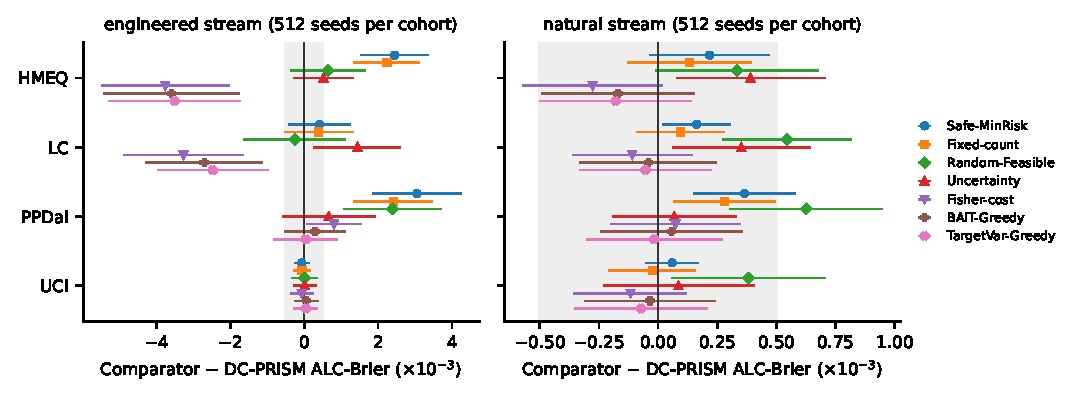
\includegraphics[width=\linewidth]{figures/supplement_v5_online.pdf}
 \caption{Comparator minus DC-PRISM ALC-Brier with 95\% simultaneous intervals over the 56-test family (512 seeds per cell); positive favors DC-PRISM. Gray band: $\pm5\times10^{-4}$. Note the different horizontal scales.}
 \label{fig:replay}
\end{figure}

\paragraph{Results.} With this power the replay becomes informative (Table~\ref{tab:replay}, Fig.~\ref{fig:replay}). On the engineered stream DC-PRISM is materially better than the quantity-oriented references on HMEQ (Safe-MinRisk $2.4$, fixed count $2.2$) and PPDai ($3.1$, $2.4$, and Random $2.4$), but materially \emph{worse} than Fisher-cost, BAIT-greedy and TargetVar-greedy on HMEQ ($3.5$--$3.8$) and LendingClub ($2.5$--$3.3$), where those policies also take fewer labels and incur less exploration loss; on UCI Credit all seven differences lie inside the material band. On the natural stream no comparison is material: 19 of 28 lie inside the band and six favor DC-PRISM by less than $0.65$ (all $\times10^{-3}$). ROC-AUC, a secondary family, shows the same pattern: DC-PRISM gains $0.005$ over the quantity references on engineered HMEQ and $0.010$--$0.015$ over Random and Uncertainty on engineered PPDai, and loses $0.005$ to Fisher-cost on engineered LendingClub, and no natural-stream AUC difference is material. Realized adverse exposure exceeded the envelope in 0--4 of 40{,}960 acquisition rounds per policy (2 for DC-PRISM; Clopper--Pearson upper bound $\le2.2\times10^{-4}$), and averaged 14--19\% of the envelope. The replay thus agrees with Secs.~\ref{sec:controlled}--\ref{sec:realx}: on real outcomes the pending-aware comparison beats taking the most labels on two engineered cohorts, but it loses to direct information-greedy selection on two others, and the natural stream does not separate the policies.

\paragraph{Validity of the replay.} The replay inherits two limits of public credit data. LendingClub, and to our knowledge the other cohorts, contain only approved loans, so ``candidates'' are drawn from a population that was already screened and the outcomes of rejected applicants are missing~\cite{crook2004reject}; the replay therefore tests acquisition among previously acceptable applicants, not the full selective-label problem. Splits are random rather than calendar-based, and the delays of one and two rounds are stylized.

\section{Related Work}
\label{sec:related}
\paragraph{Value of information and evaluation.} EVPI and the expected value of sample information are classical in decision analysis~\cite{howard1966information,raiffa1961applied}, and the upward bias of selecting the best of noisy estimates is known as the optimizer's curse~\cite{smith2006optimizer} or selection bias in model selection~\cite{cawley2010overfitting}. Krause and Guestrin~\cite{krause2005near} optimize value of information under budgets. We use these ideas not to select, but to evaluate acquisition rules: the foresight term is an EVPI over a visible family, and cross-fitting~\cite{chernozhukov2018double} supplies the lower side of the bracket.

\paragraph{Experimental design and active learning.} Bayesian experimental design~\cite{chaloner1995bayesian} and active learning~\cite{cohn1996active,settles2009active} choose observations to improve a model, with criteria from uncertainty~\cite{lewis1994sequential} and transductive design~\cite{yu2006transductive} to Fisher information~\cite{ash2021fishing}, gradient diversity~\cite{ash2020badge}, mutual information~\cite{kirsch2019batchbald,bickfordsmith2023prediction} and decision loss~\cite{huang2026loss}; budgeted variants handle heterogeneous costs~\cite{tomanek2010cost,morato2025conbatch}, and submodular maximization under knapsack constraints underlies greedy batch selection~\cite{sviridenko2004note}. These methods supply the information geometry we use.

\paragraph{Selective labels, safety and delay.} Selective-label work formalizes outcomes revealed only by favorable decisions~\cite{lakkaraju2017selective}; Wei~\cite{wei2021selective}, Kilbertus et al.~\cite{kilbertus2020fair} and Keswani et al.~\cite{keswani2024partial} trade exploration against utility, fairness or coverage, and logged data can seed further experimentation~\cite{yan2018logged}. Reject inference corrects for the missing outcomes of rejected applicants~\cite{crook2004reject}. Safe exploration~\cite{sui2015safe}, safe active learning~\cite{schreiter2015safe} and conservative bandits~\cite{wu2016conservative} constrain exploration by a safety or baseline requirement, and delayed-feedback learning~\cite{joulani2013delayed,chapelle2014delayed} and latency-aware active learning~\cite{pham2022latency} handle late outcomes. 

\section{Discussion and Conclusion}
\label{sec:conclusion}
Hindsight comparisons with the best realized set are a natural way to argue that a rule ``leaves value on the table''; our protocol shows when they mislead. In controlled worlds built around directional pending information, most hindsight headroom is deployable in every generator variant we tried, and a target-weighted proxy evaluated over a reference-anchored family captures much of it with fewer labels. Foresight itself is a roughly constant label-noise floor, so its share is large exactly where real differences are small. On real credit covariates, most of the same headroom is EVPI; the deployable remainder grows with coverage gaps and is partly identified by the same proxy, but a conservative decision rule leaves it largely unused. In a well-powered replay on real outcomes the same rule beats quantity-oriented references on two cohorts and loses to information-greedy selection on two others. For practitioners, the actionable conclusion is the protocol: hindsight headroom is a poor guide to what an acquisition rule can still gain.

\paragraph{Limitations.} Real-covariate outcomes are generated from known probabilities, because measuring $H_{\mathrm{pre}}$ requires them. Replay uses processed cohorts of approved loans with random splits (Sec.~\ref{sec:replay}). The envelope's guarantee requires simultaneous coverage by $q$, which our scores do not ensure, although realized exceedance was far below $\alpha$. BAIT-greedy (forward step only) and TargetVar-greedy (a Laplace approximation to EPIG) are adaptations, not full reimplementations. Constants were inherited rather than derived; the perturbation and sensitivity studies bound, but do not remove, this concern.

\paragraph{Outlook.} Two directions follow: reporting pre-outcome rather than hindsight headroom whenever acquisition rules are evaluated, and diagnosing proxy reliability from visible information so that conservatism is applied only where the proxy ranks poorly. Code, frozen protocols with commit hashes, aggregate results and verifiers are available in an anonymized repository.

\bibliographystyle{splncs04}
\bibliography{refs}
\end{document}
